%---------------------------------------------------------------------------------------------------
% Hauptteil
%---------------------------------------------------------------------------------------------------
\section{Hauptteil} 

\subsection{Der Token Ring Algorithmus}
Der Token Ring Algorithmus ist ein Wahlalgorithmus der von Chang und Roberts 1979 entworfen wurde. Er kann verteilt auf mehreren Clienten verwendet werden die in einer Ring-Topologie miteinander verbunden sind. Das Ziel des Algorithmus ist, bei Ausfall des Master-Clienten im Netz einen neuen zu wählen.

\subsubsection*{Voraussetzungen}
Damit der Algorithmus auf eine Ring-Topologie angewandt werden kann, müssen folgende Voraussetzungen im Netz gegeben sein:
\begin{itemize}
	\item Jeder Client kennt seinen Nachfolger
	\item Jeder Client ist mit seinem Nachfolger verbunden, sodass er mit ihm kommunizieren kann
	\item Jeder Client hat eine eindeutige ID
	\item Jeder Client kennt die gesamte Ring-Topologie
\end{itemize}

\subsubsection*{Ablauf}
\label{sec:algorithm_process}
Der Algorithmus startet wenn der Master-Client ausfällt. Der Vorgänger des ausgefallenen Master-Clients baut eine Verbindung zum Nachfolger des ausgefallenen Master-Clients auf, sodass die Ring-Topologie wieder vollständig ist.

Der Client, der den Ausfall bemerkt, startet die Wahl in dem er seinem Nachfolger eine Nachricht mit seiner ID und der Info dass es sich um eine Wahl handelt schickt. Dieser nimmt die Nachricht und überprüft ob seine eigene ID darin vor kommt. Falls nicht, hängt er seine eigene ID hinten an und schickt die vervollständigte Nachricht an seinen Nachfolger.

Wenn ein Client feststellt, dass seine eigene ID bereits in der Nachricht vorhanden ist, nimmt er die höchste ID aus der Liste der gesammelten IDs in der Nachricht. Anschließend sendet er eine "Gewählt"-Nachricht mit der höchsten ID an seinen Nachfolger. Der Empfänger der "Gewählt"-Nachricht merkt sich, dass der gewählte Client nun der neue Master ist und sendet seinem Nachfolger die gleiche "Gewählt"-Nachricht. Jeder wird somit benachrichtigt was die höchste ID ist. Kommt die "Gewählt" Nachricht wieder am Initiator der "Gewählt"-Nachricht an, wird die Wahl erfolgreich beendet und der Algorithmus ist terminiert.

\subsubsection*{Eigenschaften}
 Laufzeit
Welche Grundlegenden Eigenschaften hat der Algorithmus
was tut er und warum, wofür?

\subsection{Spezifikation}
Damit ein Modell erstellt werden kann, das den Algorithmus abbildet, müssen zunächst die charakteristischen Eigenschaften des Algorithmus bestimmt werden.

Der Algorithmus (s. Abschnitt \ref{sec:algorithm_process}) lässt sich in folgende drei Phasen einteilen:
\begin{description}
\item[Phase 1:] Ein Client bemerkt den Ausfall des bisherigen Masters
\item[Phase 2:] Sammeln aller beteiligten Client-IDs
\item[Phase 3:] Bekanntgeben des neuen Masters
\end{description}

Der jeweilige Ablauf der Phasen lässt sich mit folgenden Punkten spezifieren:

\begin{table}
\begin{tabular}{|c|p{7,6cm}|c|}
\hline Phase & Eigenschaft & Nr.\\ 
\hline Phase 1: Master-Ausfall bemerkt & Sendet Nachricht zum Wählen und hängt seine eigene ID daran & 1\\ 
\hline \multirow{3}*{Phase 2: Wahl} & Client, der Wahl-Nachricht erhält, hängt seine eigene ID an die Nachricht & 2\\ 
\cline{2-3} & Client sendet die erweiterte Nachricht an seinen Nachfolger & 3\\ 
\cline{2-3} & Sobald ein Client eine Wahl-Nachricht erhält, in der seine eigene ID bereits enthalten ist, geht der Algorithmus in Phase 3 über & 4\\ 
\hline \multirow{3}{*}{Phase 3: Neuen Master mitteilen} & Der Client, der feststellt, dass Phase 2 vorbei ist, sendet eine Nachricht mit dem neuen Master an seinen Nachfolger & 5\\
\cline{2-3} & Ein Client, der die Nachricht über einen Master erhält, merkt sich den neuen Master & 6\\ 
\cline{2-3} & Ein Client, der die Nachricht über einen Master erhält, teilt seinem Nachfolger diese Nachricht mit & 7\\
\cline{2-3} & Sobald der Client, der Phase 3 eingeleitet hat, die Nachricht über den neuen Master erhalten hat, terminiert der Algorithmus & 8\\
\hline 
\end{tabular}
\caption{Spezifikation der Phasen des Algorithmus}
\label{table: algorithm_specification} 
\end{table}

\subsection{Modellierung}
\label{sec:model}
Wie haben wir ihn modelliert
-Gefärbtes netz
- Ids
- Guards
Erklären an wo die spezifizierten Punkte im Netz zu finden sind.

\subsubsection{Das Netz}
Hier Netzbild einbinden




\subsection{Korrektheit}
Um zu zeigen, dass das erstellte Modell dem Algorithmus entspricht, wird im Folgenden die Korrektheit bewiesen. Dazu wird die Existenz der spezifizierten Eigenschaften aus Tabelle \ref{table: algorithm_specification} im erstellten Petri-Netz durch CTL-Ausdrücke geprüft.

\subsubsection{Umwandlung CPN zu PN}
Das in Abschnitt \ref{sec:model} erstellte Modell ist ein farbiges Petri-Netz (engl: Colored Petri Net, Kurz: CPN), daher lässt sich darauf nicht die CTL anwenden. Um die CTL verwenden zu können, muss vorher das erstellte Netz in ein einfaches Petri-Netz umgewandelt werden.

Das Modell-CPN verwendet einige Transition-Guards und einen Datentyp mit einem begrenzten Wertraum. Diese Logik ist nicht in einfachen Petri-Netzen erlaubt, daher muss sie umgewandelt werden.

Wenn im CPN auf der Stelle \textit{P1} ein Token mit dem Wert \textit{3} liegt, wird dies im PN dargestellt indem auf der Stelle \textit{P1\_3} ein Token liegt. Die Transition-Guards des CPN werden im PN durch komplexe Stellen-Transitions-Schaltungen abgebildet. Es gibt daher für \textit{P1} für jeden Wert des Datentyps eine Stelle.

Dadurch wird das PN im Vergleich zum CPN sehr groß und unübersichtlich.

\subsubsection{Erreichbarkeitsgraph}
Der Erreichbarkeitsgraph wird auf dem einfachen Petri-Netz gebildet, da die CTL-Ausdrücke auch auf dem einfachen Petri-Netz geprüft werden.

\begin{figure}[H]
\centering
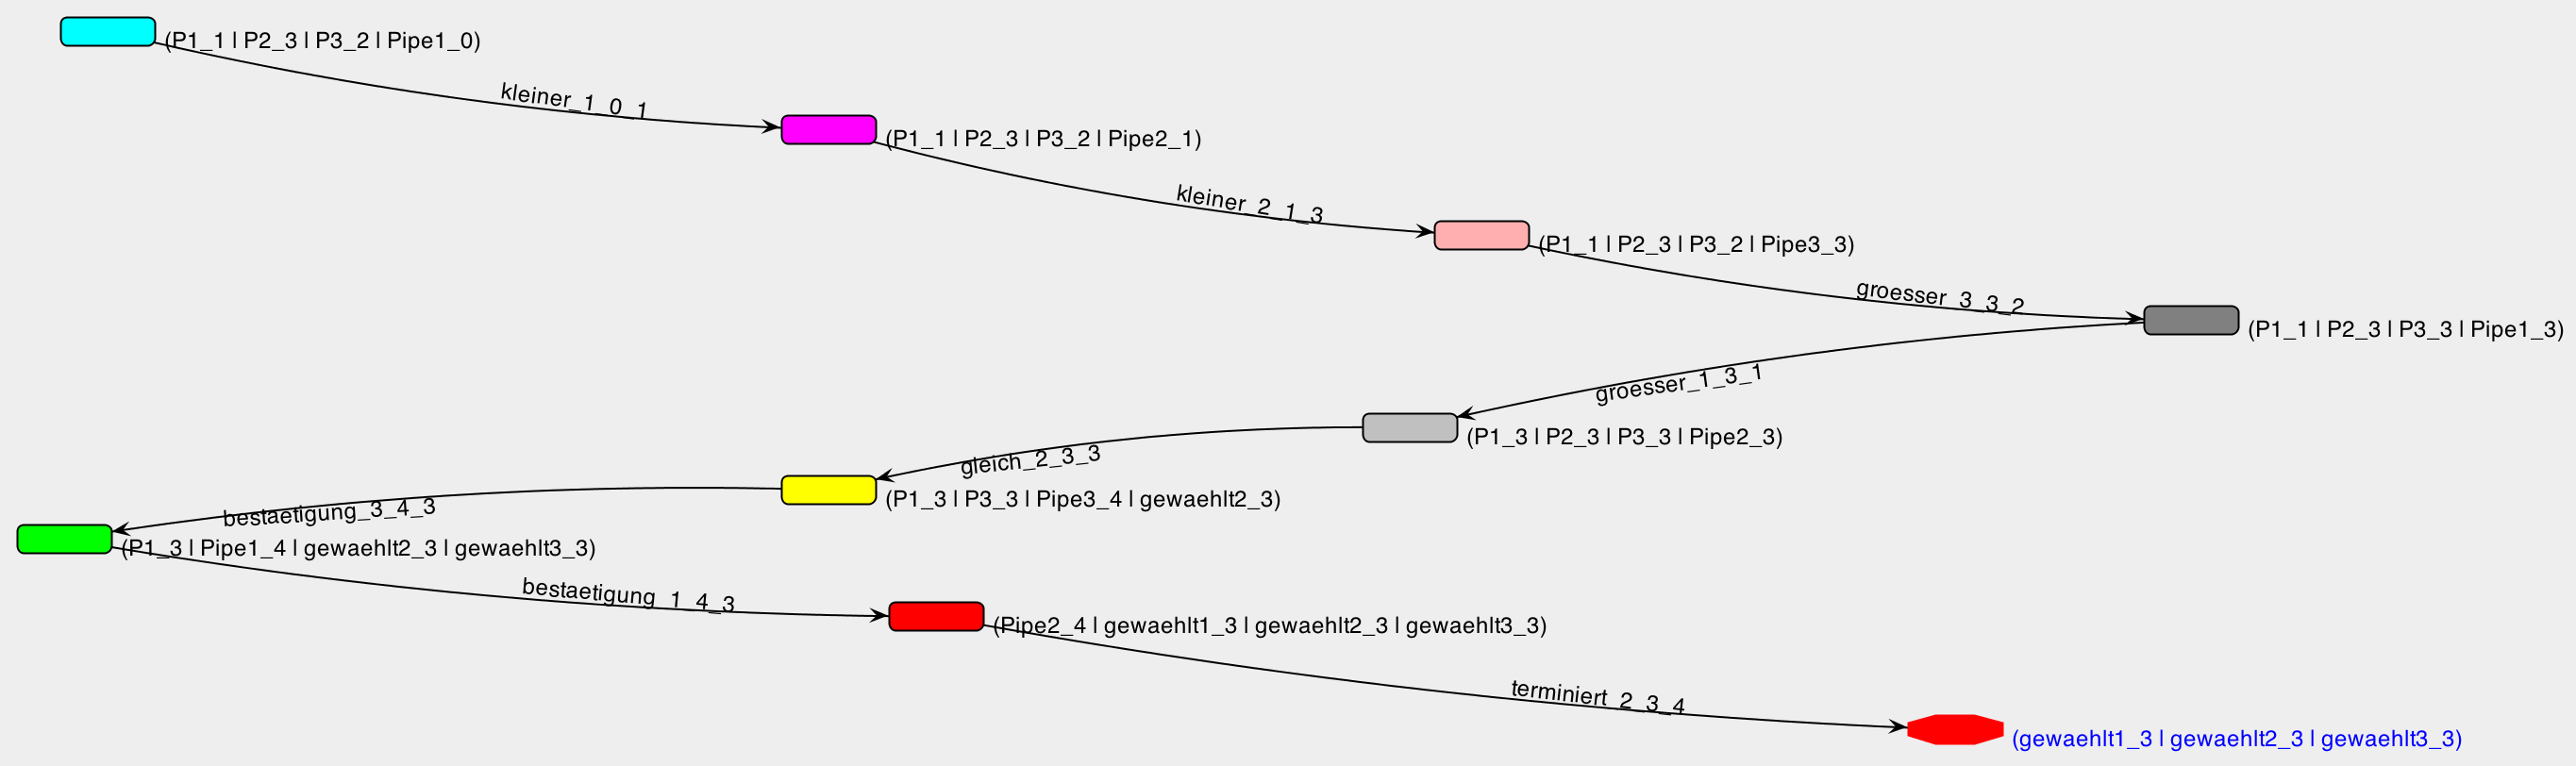
\includegraphics[width=1\linewidth]{reachibility_graph}
\caption{Erreichbarkeitsgraph des PN}
\label{fig:reachibility_graph}
\end{figure}

In Abbildung \ref{fig:reachibility_graph} ist der generierte Erreichbarkeitsgraph zu sehen. Es fällt auf, dass der Graph keine Abzweigungen hat, sondern nur einen Pfad enthält. Das bedeutet, dass der Algorithmus bei gleichen Bedingungen sich deterministisch verhält.

Würde man die Bedingungen verändern, sodass bspw. ein anderer Client den Master-Ausfall bemerkt oder ein anderer Client hat die höchste ID, dann würde sich die Reihenfolge der Kanten im Erreichbarkeitsgraph verändern und die Knoten würden andere Stellen beinhalten. Der Erreichbarkeitsgraph wäre allerdings nach wie vor geradlinig.

\subsubsection{Prüfung durch CTL}


Warum ist der Algorithmus korrekt
- Determinismus
- es kann immer nur eine Transition schalten es gibt keine Parallelität
- Erreichbarkeitsgraph zeigen und erklären
